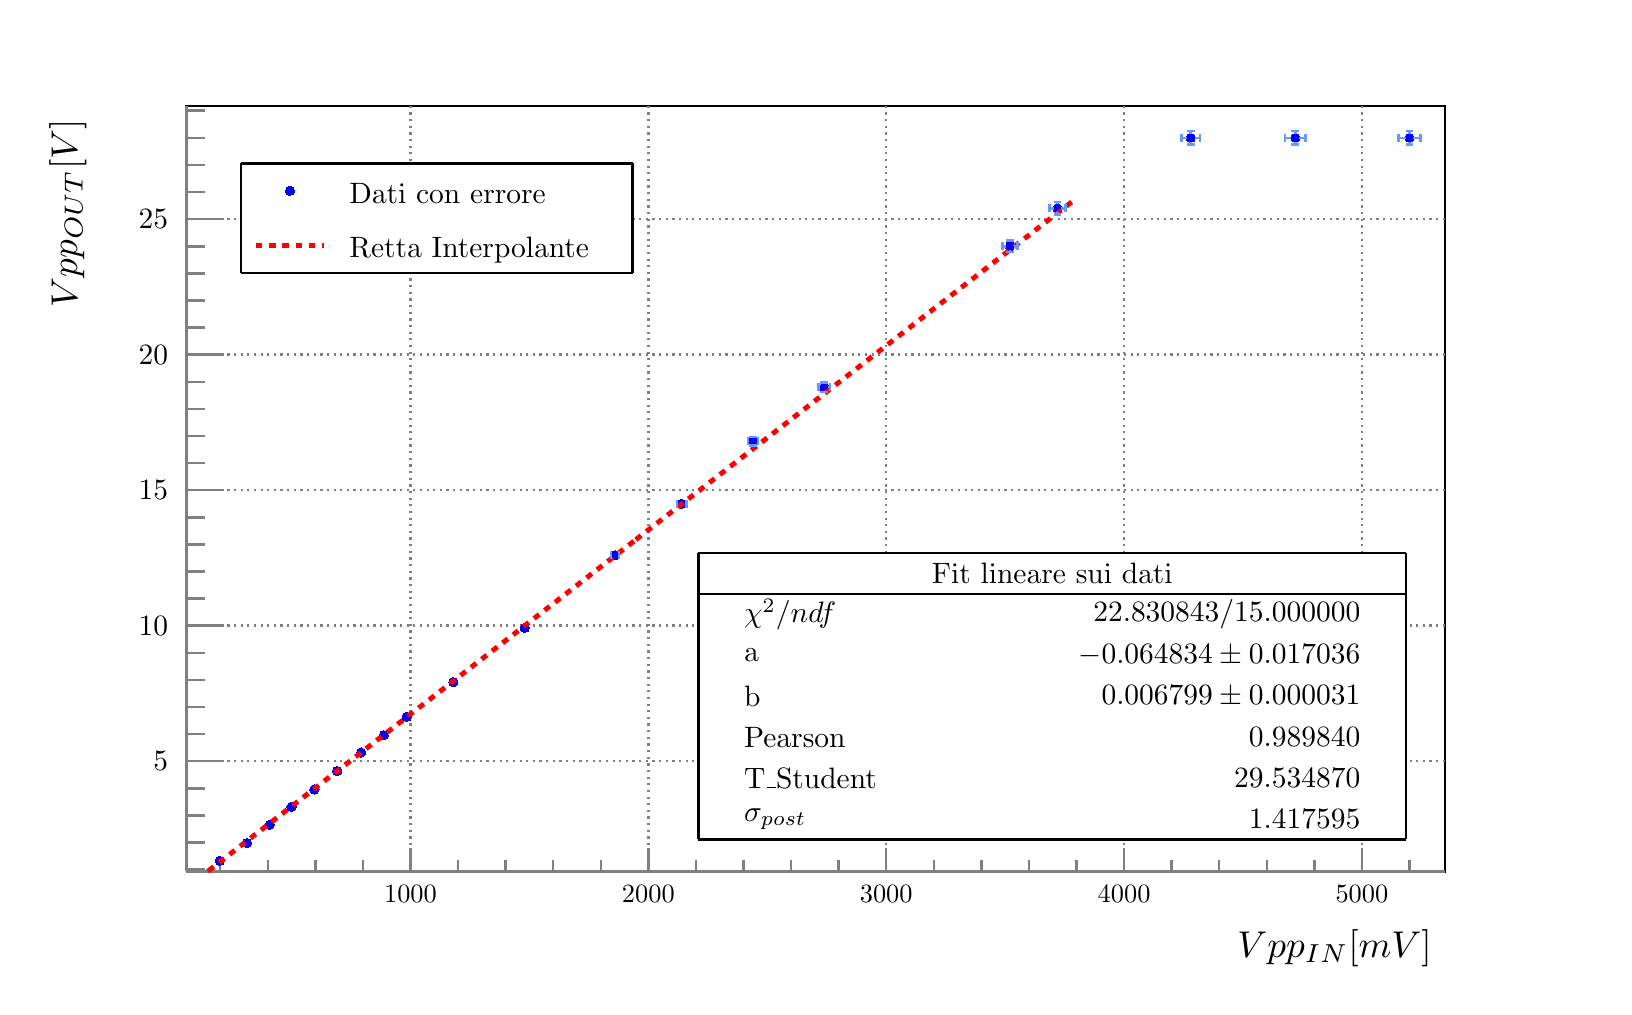
\begin{tikzpicture}
\pgfdeclareplotmark{cross} {
\pgfpathmoveto{\pgfpoint{-0.3\pgfplotmarksize}{\pgfplotmarksize}}
\pgfpathlineto{\pgfpoint{+0.3\pgfplotmarksize}{\pgfplotmarksize}}
\pgfpathlineto{\pgfpoint{+0.3\pgfplotmarksize}{0.3\pgfplotmarksize}}
\pgfpathlineto{\pgfpoint{+1\pgfplotmarksize}{0.3\pgfplotmarksize}}
\pgfpathlineto{\pgfpoint{+1\pgfplotmarksize}{-0.3\pgfplotmarksize}}
\pgfpathlineto{\pgfpoint{+0.3\pgfplotmarksize}{-0.3\pgfplotmarksize}}
\pgfpathlineto{\pgfpoint{+0.3\pgfplotmarksize}{-1.\pgfplotmarksize}}
\pgfpathlineto{\pgfpoint{-0.3\pgfplotmarksize}{-1.\pgfplotmarksize}}
\pgfpathlineto{\pgfpoint{-0.3\pgfplotmarksize}{-0.3\pgfplotmarksize}}
\pgfpathlineto{\pgfpoint{-1.\pgfplotmarksize}{-0.3\pgfplotmarksize}}
\pgfpathlineto{\pgfpoint{-1.\pgfplotmarksize}{0.3\pgfplotmarksize}}
\pgfpathlineto{\pgfpoint{-0.3\pgfplotmarksize}{0.3\pgfplotmarksize}}
\pgfpathclose
\pgfusepathqstroke
}
\pgfdeclareplotmark{cross*} {
\pgfpathmoveto{\pgfpoint{-0.3\pgfplotmarksize}{\pgfplotmarksize}}
\pgfpathlineto{\pgfpoint{+0.3\pgfplotmarksize}{\pgfplotmarksize}}
\pgfpathlineto{\pgfpoint{+0.3\pgfplotmarksize}{0.3\pgfplotmarksize}}
\pgfpathlineto{\pgfpoint{+1\pgfplotmarksize}{0.3\pgfplotmarksize}}
\pgfpathlineto{\pgfpoint{+1\pgfplotmarksize}{-0.3\pgfplotmarksize}}
\pgfpathlineto{\pgfpoint{+0.3\pgfplotmarksize}{-0.3\pgfplotmarksize}}
\pgfpathlineto{\pgfpoint{+0.3\pgfplotmarksize}{-1.\pgfplotmarksize}}
\pgfpathlineto{\pgfpoint{-0.3\pgfplotmarksize}{-1.\pgfplotmarksize}}
\pgfpathlineto{\pgfpoint{-0.3\pgfplotmarksize}{-0.3\pgfplotmarksize}}
\pgfpathlineto{\pgfpoint{-1.\pgfplotmarksize}{-0.3\pgfplotmarksize}}
\pgfpathlineto{\pgfpoint{-1.\pgfplotmarksize}{0.3\pgfplotmarksize}}
\pgfpathlineto{\pgfpoint{-0.3\pgfplotmarksize}{0.3\pgfplotmarksize}}
\pgfpathclose
\pgfusepathqfillstroke
}
\pgfdeclareplotmark{newstar} {
\pgfpathmoveto{\pgfqpoint{0pt}{\pgfplotmarksize}}
\pgfpathlineto{\pgfqpointpolar{44}{0.5\pgfplotmarksize}}
\pgfpathlineto{\pgfqpointpolar{18}{\pgfplotmarksize}}
\pgfpathlineto{\pgfqpointpolar{-20}{0.5\pgfplotmarksize}}
\pgfpathlineto{\pgfqpointpolar{-54}{\pgfplotmarksize}}
\pgfpathlineto{\pgfqpointpolar{-90}{0.5\pgfplotmarksize}}
\pgfpathlineto{\pgfqpointpolar{234}{\pgfplotmarksize}}
\pgfpathlineto{\pgfqpointpolar{198}{0.5\pgfplotmarksize}}
\pgfpathlineto{\pgfqpointpolar{162}{\pgfplotmarksize}}
\pgfpathlineto{\pgfqpointpolar{134}{0.5\pgfplotmarksize}}
\pgfpathclose
\pgfusepathqstroke
}
\pgfdeclareplotmark{newstar*} {
\pgfpathmoveto{\pgfqpoint{0pt}{\pgfplotmarksize}}
\pgfpathlineto{\pgfqpointpolar{44}{0.5\pgfplotmarksize}}
\pgfpathlineto{\pgfqpointpolar{18}{\pgfplotmarksize}}
\pgfpathlineto{\pgfqpointpolar{-20}{0.5\pgfplotmarksize}}
\pgfpathlineto{\pgfqpointpolar{-54}{\pgfplotmarksize}}
\pgfpathlineto{\pgfqpointpolar{-90}{0.5\pgfplotmarksize}}
\pgfpathlineto{\pgfqpointpolar{234}{\pgfplotmarksize}}
\pgfpathlineto{\pgfqpointpolar{198}{0.5\pgfplotmarksize}}
\pgfpathlineto{\pgfqpointpolar{162}{\pgfplotmarksize}}
\pgfpathlineto{\pgfqpointpolar{134}{0.5\pgfplotmarksize}}
\pgfpathclose
\pgfusepathqfillstroke
}
\definecolor{c}{rgb}{1,1,1};
\draw [color=c, fill=c] (0,0) rectangle (20,12.1717);
\draw [color=c, fill=c] (2.00758,1.46465) rectangle (17.9924,11.1869);
\definecolor{c}{rgb}{0,0,0};
\draw [c,line width=0.9] (2.00758,1.46465) -- (2.00758,11.1869) -- (17.9924,11.1869) -- (17.9924,1.46465) -- (2.00758,1.46465);
\definecolor{c}{rgb}{1,1,1};
\draw [color=c, fill=c] (2.00758,1.46465) rectangle (17.9924,11.1869);
\definecolor{c}{rgb}{0,0,0};
\draw [c,line width=0.9] (2.00758,1.46465) -- (2.00758,11.1869) -- (17.9924,11.1869) -- (17.9924,1.46465) -- (2.00758,1.46465);
\definecolor{c}{rgb}{0.5,0.5,0.5};
\draw [c,line width=0.9] (2.00758,1.46465) -- (17.9924,1.46465);
\draw [c,dash pattern=on 0.80pt off 1.60pt ,line width=0.9] (4.85467,11.1869) -- (4.85467,1.46465);
\draw [c,dash pattern=on 0.80pt off 1.60pt ,line width=0.9] (7.87552,11.1869) -- (7.87552,1.46465);
\draw [c,dash pattern=on 0.80pt off 1.60pt ,line width=0.9] (10.8964,11.1869) -- (10.8964,1.46465);
\draw [c,dash pattern=on 0.80pt off 1.60pt ,line width=0.9] (13.9172,11.1869) -- (13.9172,1.46465);
\draw [c,dash pattern=on 0.80pt off 1.60pt ,line width=0.9] (16.9381,11.1869) -- (16.9381,1.46465);
\draw [c,dash pattern=on 0.80pt off 1.60pt ,line width=0.9] (4.85467,11.1869) -- (4.85467,1.46465);
\draw [c,dash pattern=on 0.80pt off 1.60pt ,line width=0.9] (16.9381,11.1869) -- (16.9381,1.46465);
\draw [c,line width=0.9] (2.00758,1.46465) -- (2.00758,11.1869);
\draw [c,dash pattern=on 0.80pt off 1.60pt ,line width=0.9] (17.9924,2.86237) -- (2.00758,2.86237);
\draw [c,dash pattern=on 0.80pt off 1.60pt ,line width=0.9] (17.9924,4.58348) -- (2.00758,4.58348);
\draw [c,dash pattern=on 0.80pt off 1.60pt ,line width=0.9] (17.9924,6.30459) -- (2.00758,6.30459);
\draw [c,dash pattern=on 0.80pt off 1.60pt ,line width=0.9] (17.9924,8.02571) -- (2.00758,8.02571);
\draw [c,dash pattern=on 0.80pt off 1.60pt ,line width=0.9] (17.9924,9.74682) -- (2.00758,9.74682);
\draw [c,dash pattern=on 0.80pt off 1.60pt ,line width=0.9] (17.9924,2.86237) -- (2.00758,2.86237);
\draw [c,dash pattern=on 0.80pt off 1.60pt ,line width=0.9] (17.9924,9.74682) -- (2.00758,9.74682);
\draw [c,line width=0.9] (2.00758,1.46465) -- (17.9924,1.46465);
\draw [c,line width=0.9] (4.85467,1.75649) -- (4.85467,1.46465);
\draw [c,line width=0.9] (5.45884,1.61057) -- (5.45884,1.46465);
\draw [c,line width=0.9] (6.06301,1.61057) -- (6.06301,1.46465);
\draw [c,line width=0.9] (6.66718,1.61057) -- (6.66718,1.46465);
\draw [c,line width=0.9] (7.27135,1.61057) -- (7.27135,1.46465);
\draw [c,line width=0.9] (7.87552,1.75649) -- (7.87552,1.46465);
\draw [c,line width=0.9] (8.47969,1.61057) -- (8.47969,1.46465);
\draw [c,line width=0.9] (9.08386,1.61057) -- (9.08386,1.46465);
\draw [c,line width=0.9] (9.68803,1.61057) -- (9.68803,1.46465);
\draw [c,line width=0.9] (10.2922,1.61057) -- (10.2922,1.46465);
\draw [c,line width=0.9] (10.8964,1.75649) -- (10.8964,1.46465);
\draw [c,line width=0.9] (11.5005,1.61057) -- (11.5005,1.46465);
\draw [c,line width=0.9] (12.1047,1.61057) -- (12.1047,1.46465);
\draw [c,line width=0.9] (12.7089,1.61057) -- (12.7089,1.46465);
\draw [c,line width=0.9] (13.313,1.61057) -- (13.313,1.46465);
\draw [c,line width=0.9] (13.9172,1.75649) -- (13.9172,1.46465);
\draw [c,line width=0.9] (14.5214,1.61057) -- (14.5214,1.46465);
\draw [c,line width=0.9] (15.1255,1.61057) -- (15.1255,1.46465);
\draw [c,line width=0.9] (15.7297,1.61057) -- (15.7297,1.46465);
\draw [c,line width=0.9] (16.3339,1.61057) -- (16.3339,1.46465);
\draw [c,line width=0.9] (16.9381,1.75649) -- (16.9381,1.46465);
\draw [c,line width=0.9] (4.85467,1.75649) -- (4.85467,1.46465);
\draw [c,line width=0.9] (4.2505,1.61057) -- (4.2505,1.46465);
\draw [c,line width=0.9] (3.64633,1.61057) -- (3.64633,1.46465);
\draw [c,line width=0.9] (3.04217,1.61057) -- (3.04217,1.46465);
\draw [c,line width=0.9] (2.438,1.61057) -- (2.438,1.46465);
\draw [c,line width=0.9] (16.9381,1.75649) -- (16.9381,1.46465);
\draw [c,line width=0.9] (17.5422,1.61057) -- (17.5422,1.46465);
\definecolor{c}{rgb}{0,0,0};
\draw [anchor=base] (4.85467,1.06298) node[scale=0.953447, color=c, rotate=0]{1000};
\draw [anchor=base] (7.87552,1.06298) node[scale=0.953447, color=c, rotate=0]{2000};
\draw [anchor=base] (10.8964,1.06298) node[scale=0.953447, color=c, rotate=0]{3000};
\draw [anchor=base] (13.9172,1.06298) node[scale=0.953447, color=c, rotate=0]{4000};
\draw [anchor=base] (16.9381,1.06298) node[scale=0.953447, color=c, rotate=0]{5000};
\draw [anchor= east] (17.9924,0.490909) node[scale=1.34604, color=c, rotate=0]{$Vpp_{IN} [mV]$};
\definecolor{c}{rgb}{0.5,0.5,0.5};
\draw [c,line width=0.9] (2.00758,1.46465) -- (2.00758,11.1869);
\draw [c,line width=0.9] (2.48683,2.86237) -- (2.00758,2.86237);
\draw [c,line width=0.9] (2.2472,3.20659) -- (2.00758,3.20659);
\draw [c,line width=0.9] (2.2472,3.55082) -- (2.00758,3.55082);
\draw [c,line width=0.9] (2.2472,3.89504) -- (2.00758,3.89504);
\draw [c,line width=0.9] (2.2472,4.23926) -- (2.00758,4.23926);
\draw [c,line width=0.9] (2.48683,4.58348) -- (2.00758,4.58348);
\draw [c,line width=0.9] (2.2472,4.92771) -- (2.00758,4.92771);
\draw [c,line width=0.9] (2.2472,5.27193) -- (2.00758,5.27193);
\draw [c,line width=0.9] (2.2472,5.61615) -- (2.00758,5.61615);
\draw [c,line width=0.9] (2.2472,5.96037) -- (2.00758,5.96037);
\draw [c,line width=0.9] (2.48683,6.30459) -- (2.00758,6.30459);
\draw [c,line width=0.9] (2.2472,6.64882) -- (2.00758,6.64882);
\draw [c,line width=0.9] (2.2472,6.99304) -- (2.00758,6.99304);
\draw [c,line width=0.9] (2.2472,7.33726) -- (2.00758,7.33726);
\draw [c,line width=0.9] (2.2472,7.68148) -- (2.00758,7.68148);
\draw [c,line width=0.9] (2.48683,8.02571) -- (2.00758,8.02571);
\draw [c,line width=0.9] (2.2472,8.36993) -- (2.00758,8.36993);
\draw [c,line width=0.9] (2.2472,8.71415) -- (2.00758,8.71415);
\draw [c,line width=0.9] (2.2472,9.05837) -- (2.00758,9.05837);
\draw [c,line width=0.9] (2.2472,9.4026) -- (2.00758,9.4026);
\draw [c,line width=0.9] (2.48683,9.74682) -- (2.00758,9.74682);
\draw [c,line width=0.9] (2.48683,2.86237) -- (2.00758,2.86237);
\draw [c,line width=0.9] (2.2472,2.51815) -- (2.00758,2.51815);
\draw [c,line width=0.9] (2.2472,2.17393) -- (2.00758,2.17393);
\draw [c,line width=0.9] (2.2472,1.82971) -- (2.00758,1.82971);
\draw [c,line width=0.9] (2.2472,1.48548) -- (2.00758,1.48548);
\draw [c,line width=0.9] (2.48683,9.74682) -- (2.00758,9.74682);
\draw [c,line width=0.9] (2.2472,10.091) -- (2.00758,10.091);
\draw [c,line width=0.9] (2.2472,10.4353) -- (2.00758,10.4353);
\draw [c,line width=0.9] (2.2472,10.7795) -- (2.00758,10.7795);
\draw [c,line width=0.9] (2.2472,11.1237) -- (2.00758,11.1237);
\definecolor{c}{rgb}{0,0,0};
\draw [anchor= east] (1.90758,2.86237) node[scale=1.06562, color=c, rotate=0]{5};
\draw [anchor= east] (1.90758,4.58348) node[scale=1.06562, color=c, rotate=0]{10};
\draw [anchor= east] (1.90758,6.30459) node[scale=1.06562, color=c, rotate=0]{15};
\draw [anchor= east] (1.90758,8.02571) node[scale=1.06562, color=c, rotate=0]{20};
\draw [anchor= east] (1.90758,9.74682) node[scale=1.06562, color=c, rotate=0]{25};
\draw [anchor= east] (0.502525,11.1869) node[scale=1.34604, color=c, rotate=90]{$Vpp_{OUT} [V]$};
\definecolor{c}{rgb}{0,0,1};
\foreach \P in {(2.43196,1.59908), (2.77633,1.82282), (3.06633,2.05689), (3.34425,2.28408), (3.63425,2.50438), (3.92425,2.73845), (4.22634,2.97252), (4.51634,3.19283), (4.80634,3.4269), (5.39843,3.8675), (6.30468,4.55595), (7.4526,5.47846),
 (8.29844,6.13248), (9.20469,6.92419), (10.1109,7.61264), (12.4672,9.4026), (13.0714,9.88451), (14.763,10.7795), (16.0922,10.7795), (17.5422,10.7795)}{\draw[mark options={color=c,fill=c},mark size=1.681682pt, line width=0.000000pt, mark=*] plot
 coordinates {\P};}
\definecolor{c}{rgb}{1,0,0};
\draw [c,dash pattern=on 2.40pt off 2.40pt ,line width=1.8] (2.28006,1.46465) -- (2.29021,1.47251);
\draw [c,dash pattern=on 2.40pt off 2.40pt ,line width=1.8] (2.29021,1.47251) -- (2.40327,1.5601) -- (2.51632,1.64768) -- (2.62938,1.73527) -- (2.74243,1.82285) -- (2.85549,1.91044) -- (2.96854,1.99802) -- (3.08159,2.08561) -- (3.19465,2.17319) --
 (3.3077,2.26078) -- (3.42076,2.34836) -- (3.53381,2.43595) -- (3.64687,2.52353) -- (3.75992,2.61112) -- (3.87298,2.6987) -- (3.98603,2.78629) -- (4.09909,2.87387) -- (4.21214,2.96146) -- (4.3252,3.04904) -- (4.43825,3.13663) -- (4.55131,3.22421) --
 (4.66436,3.3118) -- (4.77741,3.39938) -- (4.89047,3.48697) -- (5.00352,3.57455) -- (5.11658,3.66214) -- (5.22963,3.74972) -- (5.34269,3.83731) -- (5.45574,3.9249) -- (5.5688,4.01248) -- (5.68185,4.10007) -- (5.79491,4.18765) -- (5.90796,4.27524) --
 (6.02102,4.36282) -- (6.13407,4.45041) -- (6.24712,4.53799) -- (6.36018,4.62558) -- (6.47323,4.71316) -- (6.58629,4.80075) -- (6.69934,4.88833) -- (6.8124,4.97592) -- (6.92545,5.0635) -- (7.03851,5.15109) -- (7.15156,5.23867) -- (7.26462,5.32626) --
 (7.37767,5.41384) -- (7.49073,5.50143) -- (7.60378,5.58901) -- (7.71684,5.6766);
\draw [c,dash pattern=on 2.40pt off 2.40pt ,line width=1.8] (7.71684,5.6766) -- (7.82989,5.76418) -- (7.94294,5.85177) -- (8.056,5.93935) -- (8.16905,6.02694) -- (8.28211,6.11452) -- (8.39516,6.20211) -- (8.50822,6.28969) -- (8.62127,6.37728) --
 (8.73433,6.46486) -- (8.84738,6.55245) -- (8.96044,6.64003) -- (9.07349,6.72762) -- (9.18655,6.8152) -- (9.2996,6.90279) -- (9.41265,6.99037) -- (9.52571,7.07796) -- (9.63876,7.16554) -- (9.75182,7.25313) -- (9.86487,7.34071) -- (9.97793,7.4283) --
 (10.091,7.51588) -- (10.204,7.60347) -- (10.3171,7.69106) -- (10.4301,7.77864) -- (10.5432,7.86623) -- (10.6563,7.95381) -- (10.7693,8.0414) -- (10.8824,8.12898) -- (10.9954,8.21657) -- (11.1085,8.30415) -- (11.2215,8.39174) -- (11.3346,8.47932) --
 (11.4476,8.56691) -- (11.5607,8.65449) -- (11.6737,8.74208) -- (11.7868,8.82966) -- (11.8999,8.91725) -- (12.0129,9.00483) -- (12.126,9.09242) -- (12.239,9.18) -- (12.3521,9.26759) -- (12.4651,9.35517) -- (12.5782,9.44276) -- (12.6912,9.53034) --
 (12.8043,9.61793) -- (12.9173,9.70551) -- (13.0304,9.7931) -- (13.1435,9.88068) -- (13.2565,9.96827);
\definecolor{c}{rgb}{0.4,0.6,1};
\draw [c,line width=0.9] (7.40209,5.47846) -- (7.40067,5.47846);
\draw [c,line width=0.9] (7.40067,5.42796) -- (7.40067,5.52897);
\draw [c,line width=0.9] (7.5031,5.47846) -- (7.50453,5.47846);
\draw [c,line width=0.9] (7.50453,5.42796) -- (7.50453,5.52897);
\draw [c,line width=0.9] (8.24793,6.13248) -- (8.23959,6.13248);
\draw [c,line width=0.9] (8.23959,6.08198) -- (8.23959,6.18299);
\draw [c,line width=0.9] (8.34894,6.13248) -- (8.35728,6.13248);
\draw [c,line width=0.9] (8.35728,6.08198) -- (8.35728,6.18299);
\draw [c,line width=0.9] (9.15419,6.92419) -- (9.13833,6.92419);
\draw [c,line width=0.9] (9.13833,6.87369) -- (9.13833,6.9747);
\draw [c,line width=0.9] (9.25519,6.92419) -- (9.27105,6.92419);
\draw [c,line width=0.9] (9.27105,6.87369) -- (9.27105,6.9747);
\draw [c,line width=0.9] (9.20469,6.9747) -- (9.20469,6.97837);
\draw [c,line width=0.9] (9.15419,6.97837) -- (9.25519,6.97837);
\draw [c,line width=0.9] (9.20469,6.87369) -- (9.20469,6.87002);
\draw [c,line width=0.9] (9.15419,6.87002) -- (9.25519,6.87002);
\draw [c,line width=0.9] (10.0604,7.61264) -- (10.037,7.61264);
\draw [c,line width=0.9] (10.037,7.56213) -- (10.037,7.66314);
\draw [c,line width=0.9] (10.1614,7.61264) -- (10.1849,7.61264);
\draw [c,line width=0.9] (10.1849,7.56213) -- (10.1849,7.66314);
\draw [c,line width=0.9] (10.1109,7.66314) -- (10.1109,7.67237);
\draw [c,line width=0.9] (10.0604,7.67237) -- (10.1614,7.67237);
\draw [c,line width=0.9] (10.1109,7.56213) -- (10.1109,7.55291);
\draw [c,line width=0.9] (10.0604,7.55291) -- (10.1614,7.55291);
\draw [c,line width=0.9] (12.4167,9.4026) -- (12.3733,9.4026);
\draw [c,line width=0.9] (12.3733,9.35209) -- (12.3733,9.4531);
\draw [c,line width=0.9] (12.5177,9.4026) -- (12.5611,9.4026);
\draw [c,line width=0.9] (12.5611,9.35209) -- (12.5611,9.4531);
\draw [c,line width=0.9] (12.4672,9.4531) -- (12.4672,9.47706);
\draw [c,line width=0.9] (12.4167,9.47706) -- (12.5177,9.47706);
\draw [c,line width=0.9] (12.4672,9.35209) -- (12.4672,9.32813);
\draw [c,line width=0.9] (12.4167,9.32813) -- (12.5177,9.32813);
\draw [c,line width=0.9] (13.0209,9.88451) -- (12.9724,9.88451);
\draw [c,line width=0.9] (12.9724,9.834) -- (12.9724,9.93501);
\draw [c,line width=0.9] (13.1219,9.88451) -- (13.1704,9.88451);
\draw [c,line width=0.9] (13.1704,9.834) -- (13.1704,9.93501);
\draw [c,line width=0.9] (13.0714,9.93501) -- (13.0714,9.96299);
\draw [c,line width=0.9] (13.0209,9.96299) -- (13.1219,9.96299);
\draw [c,line width=0.9] (13.0714,9.834) -- (13.0714,9.80602);
\draw [c,line width=0.9] (13.0209,9.80602) -- (13.1219,9.80602);
\draw [c,line width=0.9] (14.7125,10.7795) -- (14.6454,10.7795);
\draw [c,line width=0.9] (14.6454,10.729) -- (14.6454,10.83);
\draw [c,line width=0.9] (14.8135,10.7795) -- (14.8807,10.7795);
\draw [c,line width=0.9] (14.8807,10.729) -- (14.8807,10.83);
\draw [c,line width=0.9] (14.763,10.83) -- (14.763,10.8655);
\draw [c,line width=0.9] (14.7125,10.8655) -- (14.8135,10.8655);
\draw [c,line width=0.9] (14.763,10.729) -- (14.763,10.6935);
\draw [c,line width=0.9] (14.7125,10.6935) -- (14.8135,10.6935);
\draw [c,line width=0.9] (16.0417,10.7795) -- (15.9635,10.7795);
\draw [c,line width=0.9] (15.9635,10.729) -- (15.9635,10.83);
\draw [c,line width=0.9] (16.1427,10.7795) -- (16.2209,10.7795);
\draw [c,line width=0.9] (16.2209,10.729) -- (16.2209,10.83);
\draw [c,line width=0.9] (16.0922,10.83) -- (16.0922,10.8655);
\draw [c,line width=0.9] (16.0417,10.8655) -- (16.1427,10.8655);
\draw [c,line width=0.9] (16.0922,10.729) -- (16.0922,10.6935);
\draw [c,line width=0.9] (16.0417,10.6935) -- (16.1427,10.6935);
\draw [c,line width=0.9] (17.4917,10.7795) -- (17.4014,10.7795);
\draw [c,line width=0.9] (17.4014,10.729) -- (17.4014,10.83);
\draw [c,line width=0.9] (17.5927,10.7795) -- (17.683,10.7795);
\draw [c,line width=0.9] (17.683,10.729) -- (17.683,10.83);
\draw [c,line width=0.9] (17.5422,10.83) -- (17.5422,10.8655);
\draw [c,line width=0.9] (17.4917,10.8655) -- (17.5927,10.8655);
\draw [c,line width=0.9] (17.5422,10.729) -- (17.5422,10.6935);
\draw [c,line width=0.9] (17.4917,10.6935) -- (17.5927,10.6935);
\definecolor{c}{rgb}{1,1,1};
\draw [color=c, fill=c] (8.5101,1.86869) rectangle (17.5,5.50505);
\definecolor{c}{rgb}{0,0,0};
\draw [c,line width=0.9] (8.5101,1.86869) -- (17.5,1.86869);
\draw [c,line width=0.9] (17.5,1.86869) -- (17.5,5.50505);
\draw [c,line width=0.9] (17.5,5.50505) -- (8.5101,5.50505);
\draw [c,line width=0.9] (8.5101,5.50505) -- (8.5101,1.86869);
\draw (13.0051,5.24531) node[scale=1.06562, color=c, rotate=0]{Fit lineare sui dati};
\draw [c,line width=0.9] (8.5101,4.98557) -- (17.5,4.98557);
\draw [anchor= west] (8.9596,4.72583) node[scale=1.06562, color=c, rotate=0]{$\chi^{2} / ndf $};
\draw [anchor= east] (17.0505,4.72583) node[scale=1.06562, color=c, rotate=0]{22.830843/15.000000};
\draw [anchor= west] (8.9596,4.20635) node[scale=1.06562, color=c, rotate=0]{a        };
\draw [anchor= east] (17.0505,4.20635) node[scale=1.06562, color=c, rotate=0]{$ -0.064834\pm0.017036$};
\draw [anchor= west] (8.9596,3.68687) node[scale=1.06562, color=c, rotate=0]{b        };
\draw [anchor= east] (17.0505,3.68687) node[scale=1.06562, color=c, rotate=0]{$ 0.006799\pm0.000031$};
\draw [anchor= west] (8.9596,3.16739) node[scale=1.06562, color=c, rotate=0]{Pearson        };
\draw [anchor= east] (17.0505,3.16739) node[scale=1.06562, color=c, rotate=0]{ 0.989840};
\draw [anchor= west] (8.9596,2.64791) node[scale=1.06562, color=c, rotate=0]{T\_Student        };
\draw [anchor= east] (17.0505,2.64791) node[scale=1.06562, color=c, rotate=0]{ 29.534870};
\draw [anchor= west] (8.9596,2.12843) node[scale=1.06562, color=c, rotate=0]{$\sigma_{post}        $};
\draw [anchor= east] (17.0505,2.12843) node[scale=1.06562, color=c, rotate=0]{ 1.417595};
\definecolor{c}{rgb}{1,1,1};
\draw [color=c, fill=c] (2.70202,9.06566) rectangle (7.67677,10.4545);
\definecolor{c}{rgb}{0,0,0};
\draw [c,line width=0.9] (2.70202,9.06566) -- (7.67677,9.06566);
\draw [c,line width=0.9] (7.67677,9.06566) -- (7.67677,10.4545);
\draw [c,line width=0.9] (7.67677,10.4545) -- (2.70202,10.4545);
\draw [c,line width=0.9] (2.70202,10.4545) -- (2.70202,9.06566);
\draw [anchor=base west] (3.94571,9.95107) node[scale=1.06562, color=c, rotate=0]{Dati con errore};
\definecolor{c}{rgb}{0,0,1};
\foreach \P in {(3.32386,10.1073)}{\draw[mark options={color=c,fill=c},mark size=1.681682pt, line width=0.000000pt, mark=*] plot coordinates {\P};}
\definecolor{c}{rgb}{0,0,0};
\draw [anchor=base west] (3.94571,9.25663) node[scale=1.06562, color=c, rotate=0]{Retta Interpolante};
\definecolor{c}{rgb}{1,0,0};
\draw [c,dash pattern=on 2.40pt off 2.40pt ,line width=1.8] (2.88857,9.41288) -- (3.75915,9.41288);
\end{tikzpicture}
